\documentclass{article}
\usepackage[a4paper,top=3.5cm,bottom=5cm,left=3.8cm,right=3.8cm,marginparwidth=1.75cm]{geometry}
\usepackage{graphicx} % Required for inserting images
\usepackage{float}
\usepackage{hyperref}

\usepackage{cite}

\title{\textbf{Porject Specification}\\Natural Language Processing}
\author{Ricard Renalias \and Eric Roy}
\date{April 2025}

\begin{document}

\maketitle

\section{Introduction}

This document presents the project proposal of the Natural Language Processing (NLP) final project. This project has a 15-hour time limit (since we're doing it in a group of two people) and should be NLP-related.

\section{Motivation}

HomeAssistant \cite{homeassistant} is an open-source software framework used to automate home devices. It focuses on local control (i.e. self-hosted) and in privacy. Like many open-source applications, it is developed by volunteers.

One of the latest features of HomeAssistant is the ability to control the devices using your voice. You simply need a device that can record and stream audio to use it. HomeAssistant provides a pipeline that enables these changes, schematized like figure \ref{fig:ha-pipeline}.

\begin{figure}[H]
    \centering
    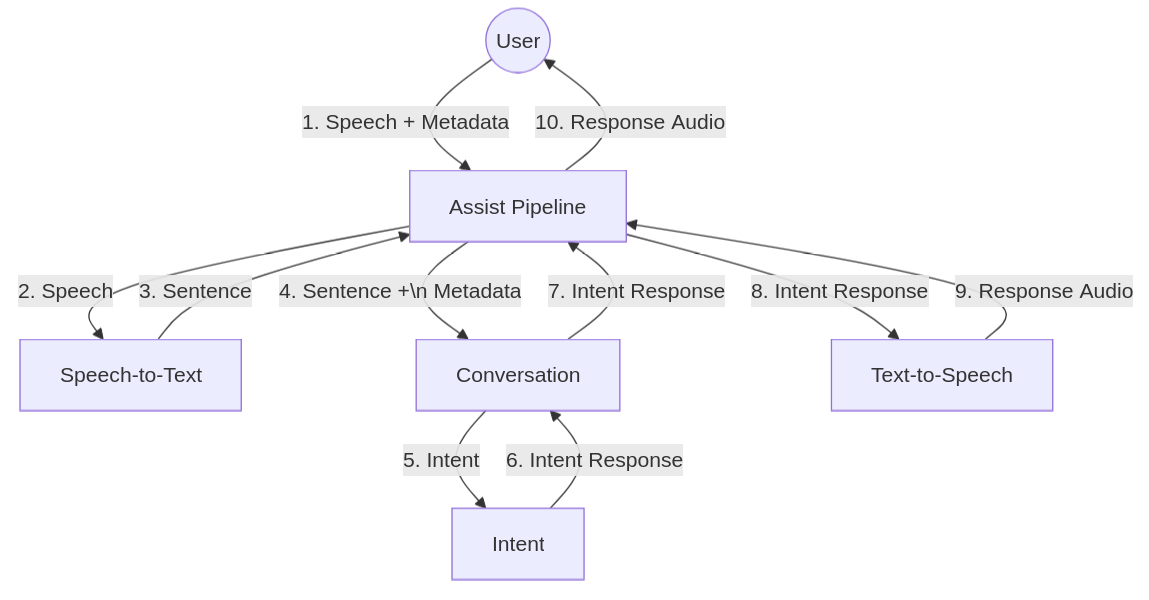
\includegraphics[width=0.75\linewidth]{pipeline_home_assistant.png}
    \caption{
    HomeAssistant's voice command's pipeline (extracted from \cite{homeassistantvoice}).
    The user connects itself to the Assist Pipeline, which will be the process handling all
    the steps. It first converts the speech to text (STT), then it uses \textit{Conversation} to
    execute the actions and get a text response, and finally, if a response is needed, it
    converts the output text to speech (TTS). This enables the possibility to still talking directly with text without changing the entire system (by removing steps 2, 3, 8 and 9.
    }
    \label{fig:ha-pipeline}
\end{figure}

Figure \ref{fig:ha-pipeline} clearly differentiates two parts during the text processing: \textit{Conversation} and \textit{Intent}. The first one will convert the natural text to a standard format (that complies with API specifications), and the second one will perform the actions and return a schematic response, that will be converted to plain text again by \textit{Conversation}.

Making a system composed by pieces has great advantages, the main one being the ability to switch parts of it without having to change everything. For example, HomeAssistant provides two different STT alternatives (although one can build their own) \cite{homeassistantspeechoptions}. \textit{Speech-to-phrase} is more lightweight and simpler, and \textit{Whisper} is more robust but also more resource-expensive. Generally, \textit{Whisper} is the option to go when talking to HomeAssistant in a non-English language.
For STT, \textit{Piper} is the default package, which provides already the vast majority of languages.

\textit{Conversation} mostly relies on pre-written sentences, which are scanned to detect the user's action. If no action is found, this means that the input sentence might not be imperative, but rather that the user asked a question. When this happens, the input is passed through an LLM instead of through \textit{Intent}, to get a meaningful response.

This system works very well with English, but some languages (like Catalan) have a lot of variations (for example: conjugations or sentence orders) which makes word scanning more complex. Moreover, inverted sentences (for example, sentences that start with 'No') might not be correctly detected. There are some solutions to this problem, but the ones supporting the Catalan language are very poor.

\section{Objective}

This project aims to set up a working system of HomeAssistant (as in figure \ref{fig:ha-pipeline}) to enable voice control in Catalan. We will use already existing parts for everyting except for the \textit{Conversation} module. The goal of this project is to replace this text scanning module with our own, more robust module. The module will have an architecture similar to figure \ref{fig:our-pipeline-ideal}.

\begin{figure}[H]
    \centering
    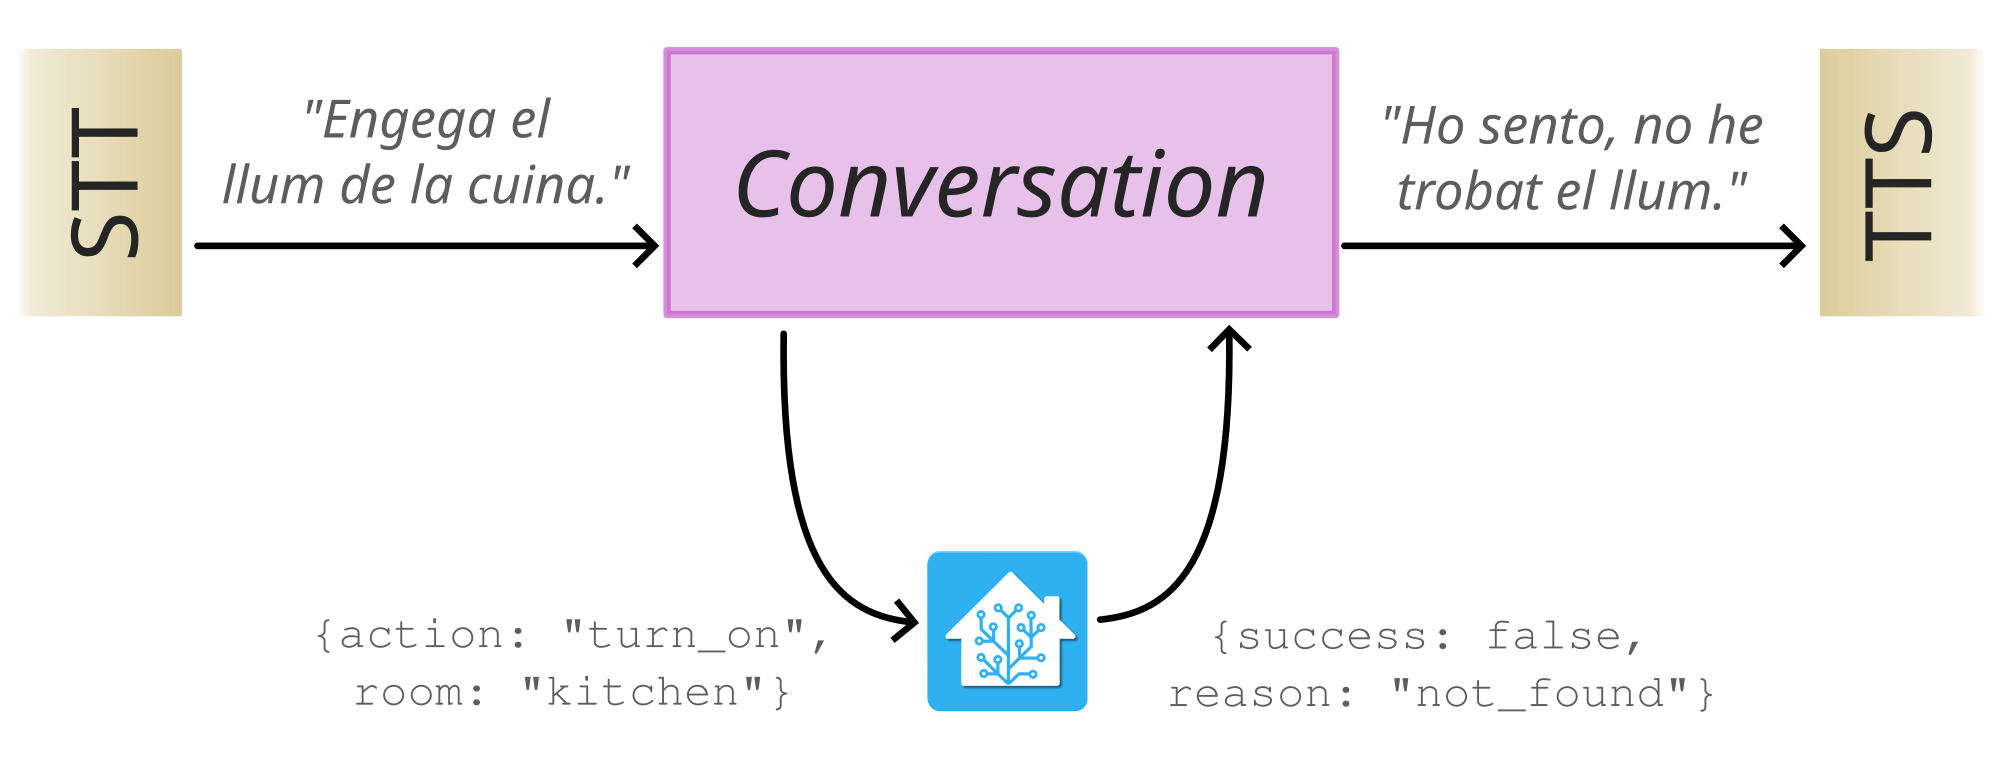
\includegraphics[width=0.95\linewidth]{drawing1.png}
    \caption{
    The \textit{Conversation} module in HomeAssistant and its main interactions with external modules. The figure contains an example of what data is sent at each step (note that the format of the payloads has been simplified to make it easier to understand). The Catalan sentences translates to "Turn on the kitchen light" and "Sorry, I haven't found the light" respectively.
    }
    \label{fig:our-pipeline-ideal}
\end{figure}

To this end, we will fine-tune an already existing model (like BERT) to accept the text as an input and generate a finite-set of outputs. It will still call \textit{Intents} to operate the automation tasks and it will make calls to a LLM, if needed, to handle more philosophical requests.

\subsection{Simplification}

Given the time available to do this project and the requirement to make a self-contained demo, we will simplify the system so it can be packaged into a few docker containers. The resulting
architecture is visible in figure \ref{fig:our-pipeline-real}.

\begin{figure}[H]
    \centering
    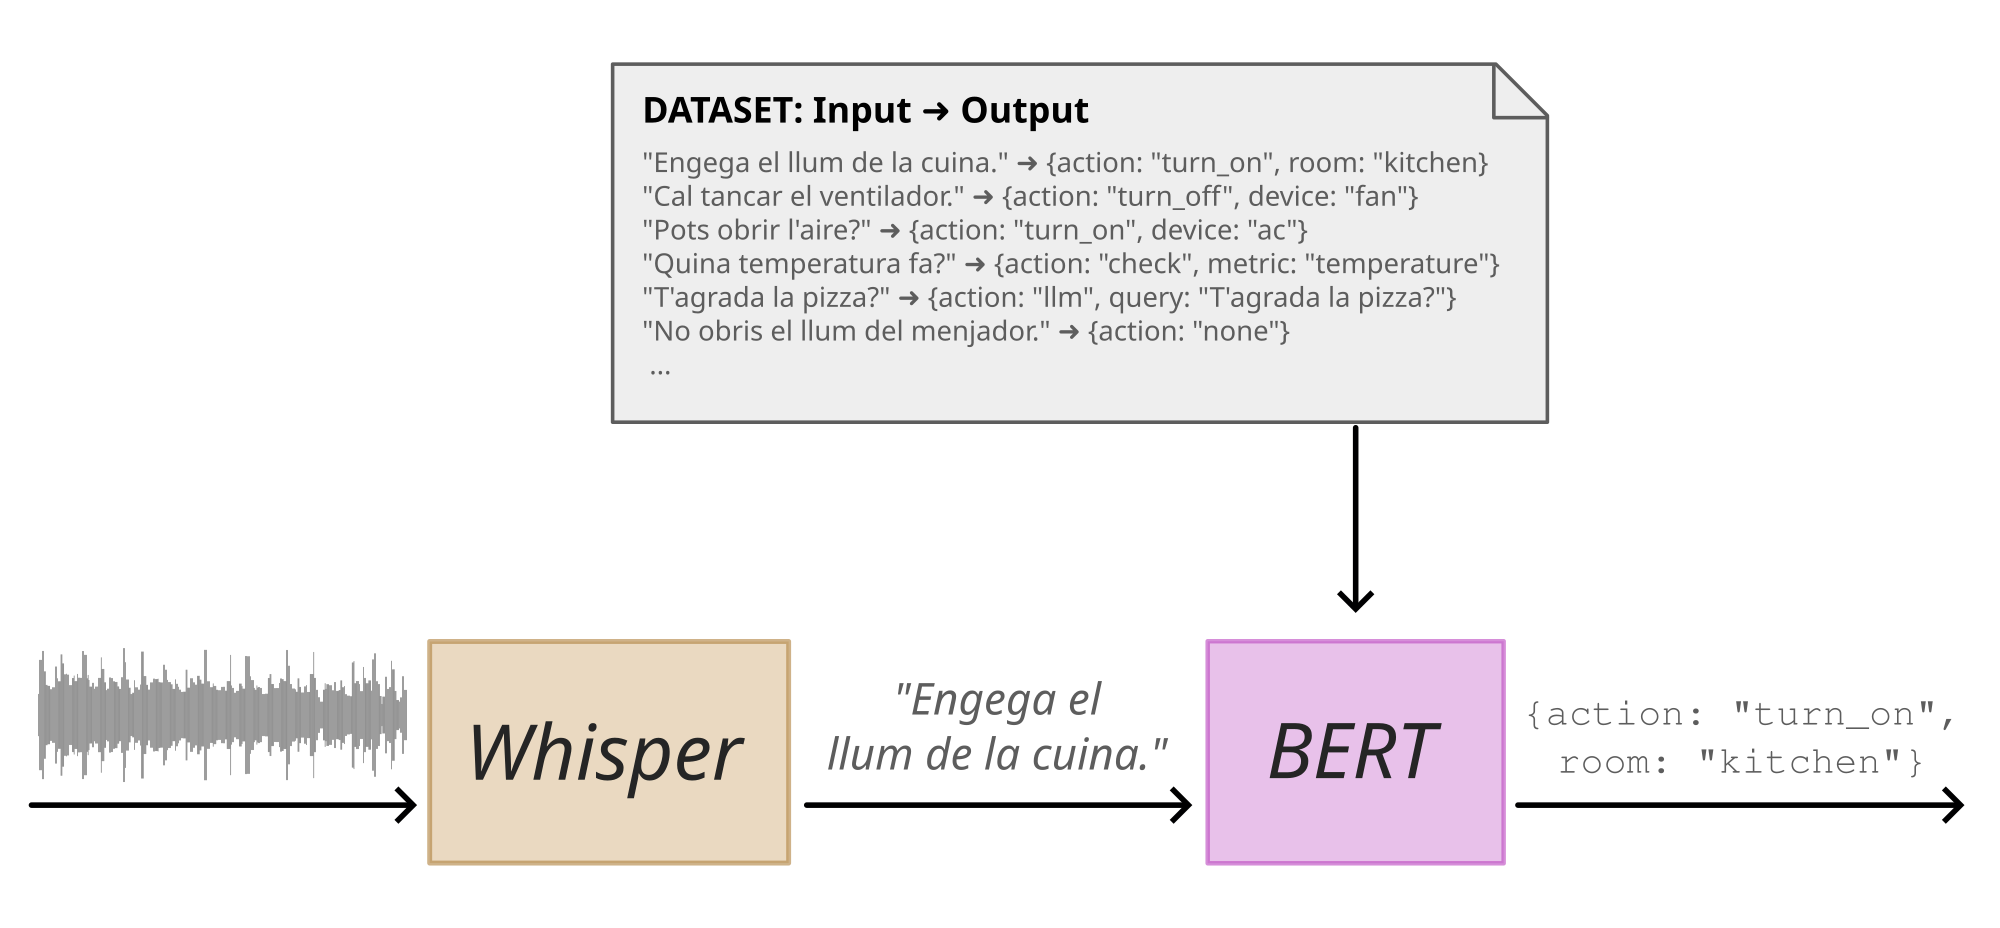
\includegraphics[width=\linewidth]{drawing2.png}
    \caption{
    Our simplification of the \textit{Conversation} module used to develop this project. Once we verify that it works correctly with this environment (that's easier to test) we will be able to easily use it in the real scenario.
    }
    \label{fig:our-pipeline-real}
\end{figure}

If we have more time available, making the system work with HomeAssistant will be a great expansion to the project.

\section{Technicalities}

This section contains some details regarding the project that are not relevant when getting a general view, but are strongly needed when trying to implement it.

\subsection{Used dataset}

To fine-tune the model we will need a dataset relating sentences and actions. We will generate the dataset ourselves (and with the help of generative tools), since fine-tuning a model does not require a lot of data. The UPC has GPU servers available to the students that we can use to train it, but we suspect it won't be that much necessary.

\subsection{Integration with HomeAssistant}

The main extension of this work is combining the created module with a real automation environment. To this end, we acquired a Voice PE device \cite{homeassistantvoicepe}, which is the analogy of the Echo Dot for HomeAssistant. However, this model is open-source and can be tuned to our liking.

\subsection{STT Tools: Whisper}

Among the two default STT that HomeAssistant provides (and also after taking a look at the State-Of-The-Art tools) we've concluded that Whisper is the tool we should use. Whisper \cite{whisper} is an automatic speech recognition Neural Network that started with only
recognizing English language, but is now robust enough to recognize Catalan. We use it
instead of Speech-To-Sentence because the latter one does not perform that good with foreign languages.

\subsection{TTS: Piper}

Piper \cite{pipertts} is a TTS system that's open-source and has Catalan voices. As a fun fact, the Catalan voices have been made by UPC researchers! This is the de-facto tool for TTS in open-source projects, and for this reason it's the default one in HomeAssistant. We'll use this one to read the responses once we integrate the entire system with HomeAssistant.

\subsection{Conversation module}

The main module of this project is the \textit{Conversation} module, which will be implemented almost from scratch. However, we'll use existing libraries and pre-trained models. The library it's most probable that we use is Python's transformers package \cite{wolf-etal-2020-transformers}. It already includes a BERT tokenizer and model generator.

\section{Methodology}

We will work in a team of two, so it's crucial to divide the work early on to guarantee no time is wasted. To this end, the first task of the project is to plan everything accordingly, and meet regularly to share progress. Some tasks will be done as a group, while others will be performed in parallel.

\subsection{Expected output and evaluation}

If all goes well, by the end of this project we should have these final results:
\begin{itemize}
    \item A functional HomeAssistant Catalan voice control in a real-life system.
    \item A self-contained demo that showcases the main module of the project.
    \item The required documentation (code and report) to share the results.
\end{itemize}

\subsection{Planning}

Table \ref{table:timetable} shows the project planning. Some of the tasks are very general and will be divided into smaller tasks. Note that times add to 15 hours.

\begin{table}[H]
\centering
\begin{tabular}{lll}
\hline
\textbf{Task} & \textbf{Time} & \\
 & Ricard & Eric \\ \hline
Research and project organisation & $1h$ & $1h$ \\
Environment setup and model creation & & $1h$ \\
Dataset creation                   & $1h$ & \\
Model training and fine-tuning   & $30min$ & $30min$ \\
Integration with whisper & & $1h$ \\
Functionnal demo preparation & & $1h$ \\
Extension: HomeAssistant integration & $3h$ & $1h$ \\
Report/readme writing and reviewing      & $2h$ & $2h$ \\
\hline
\textbf{Total time} & \textbf{7.5 hours} & \textbf{7.5 hours} \\ \hline
\end{tabular}
\caption{Project planning}
\label{table:timetable}
\end{table}


% \bibliographystyle{apalike}
\bibliographystyle{plain}
\bibliography{mybib}

\end{document}
